%!TEX root = ../Main.tex

\chapter{General discussion and final remarks}
\label{cha:discussion}
%This section wraps up by showing the relationship and importance of a comprehensive approach to data analysis, from the field, genetics, molecular biology and genomics. I will also remark how the technology and the resources have changed in the last 4 years. As at the references used at beginning where superseded during the PhD. 

%Biology is becoming interdisciplinary

%\section{Analysis and tool development for polyploid organisms}

Knowledge from  computer science can be applied to produce software for specific needs, and which can also be useful for the community. 
One of the limitations though is that most approaches are developed for diploid systems and are sometimes not compatible with polyploid species, such as wheat. 
Polyploidy adds an extra level of complexity (due to homoeologs) and in the case of wheat the large genome size also hinders certain approaches to genome analyses. Therefore bespoke tools are required to deal with this barriers. 

In this thesis we have taken advantage of developments in the technology and in resources to generate a series of solutions to many of the problems associated with polyploidy. These methods and approaches are not restricted to wheat, but can be applied and implemented to other polyploid systems.

I have discussed individual elements of project at the end of each chapter. However, looking forward my interest is to integrate this data into a single scheme. I outline this in Figure \ref{fig:discussion:allTables} and discuss it below. 

\begin{sidewaysfigure}
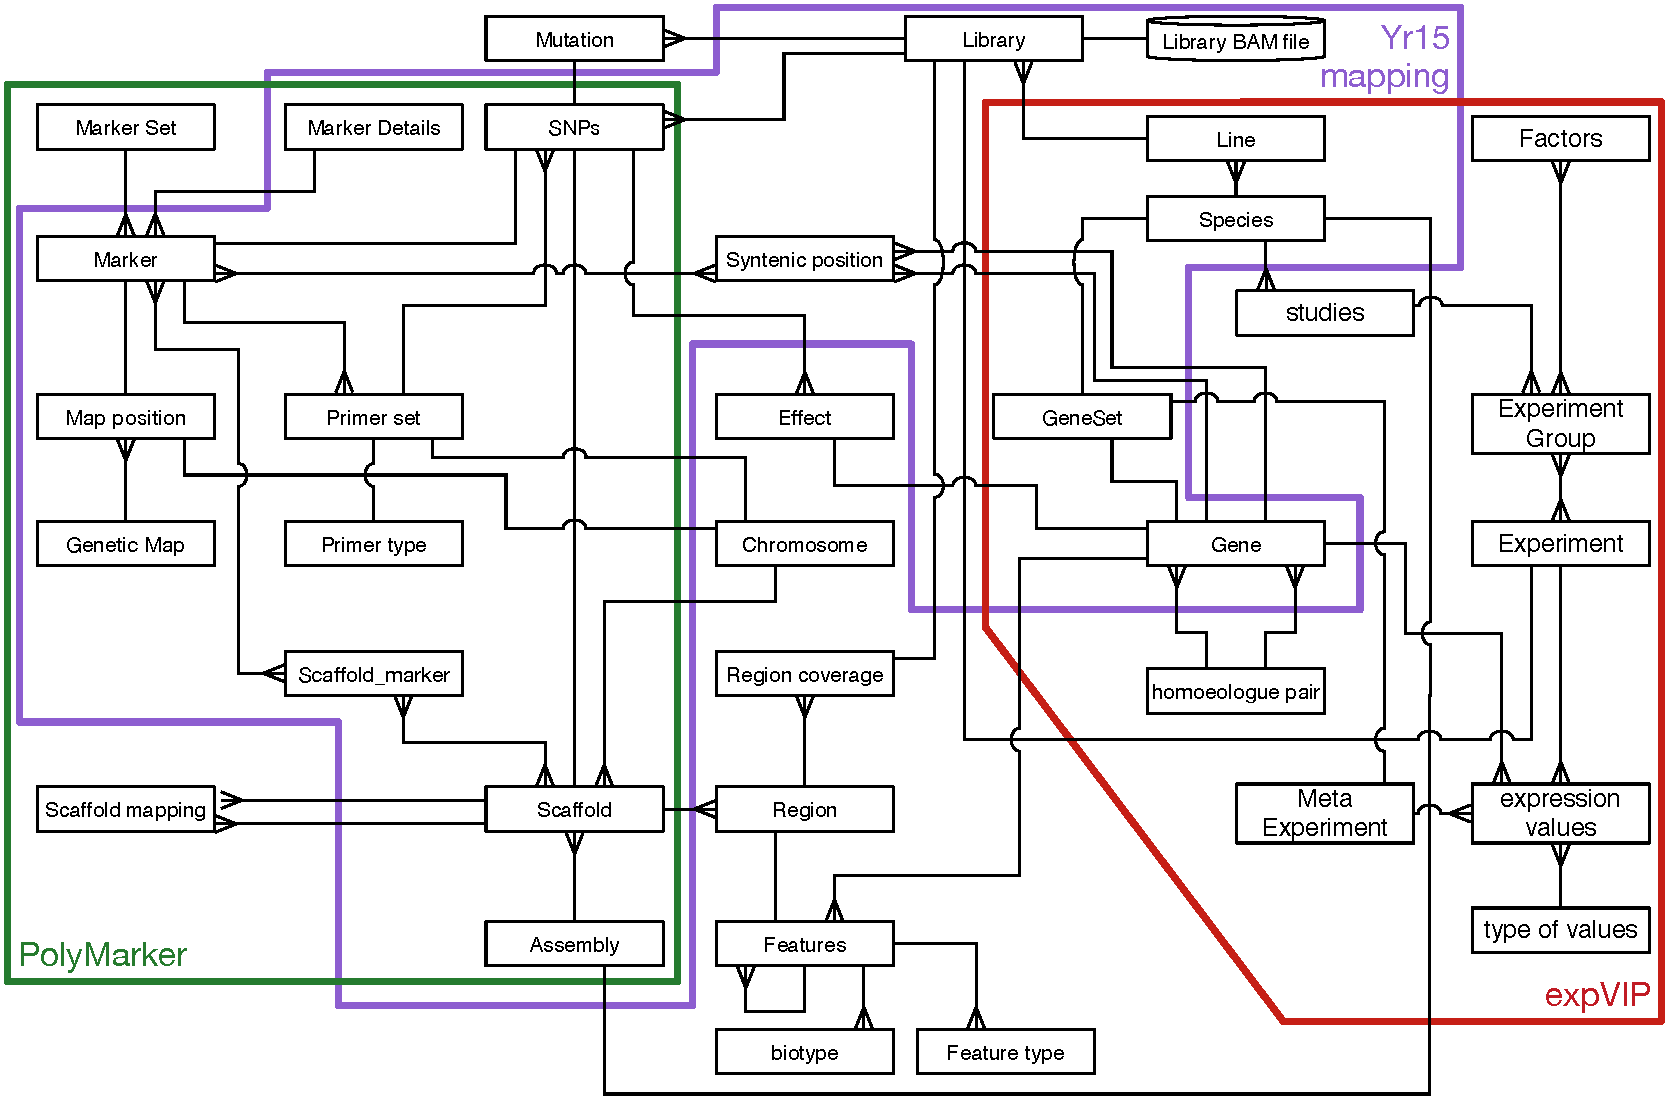
\includegraphics[width=1\textwidth]{Conclusions/Figures/CompleteDatabase.pdf}
\caption[Relational database integrating all the datasets.]{Relational database integrating all the datasets. The boxes represent the tables that contain information related to each chapter.}
\label{fig:discussion:allTables}
\end{sidewaysfigure}


\section{Integration of different genetic maps}

Genetic maps are a common starting point to start the search for a locus linked to a trait. 
For example, in Chapter \ref{yr15} previous genetics map had already identified the short arm of chromosome 1B as the locus for \acrshort{yr15} \citep{Murphy2009}.
Furthermore, I was able to confirm an enrichment of SNPs linked in the expected region thanks to the mapping of the markers included in the genetic map from \citet{Wang2014} to the \acrshort{css} scaffolds \citep{Mayer2014}. Since my initial analysis, other genetic maps with a higher resolution have been published \citep{Chapman2015, Allen2016,Winfield2016}. 
The relationship between the tables used in the genetic map is shown in Figure \ref{fig:discussion:geneticMapsTables}

\begin{figure}
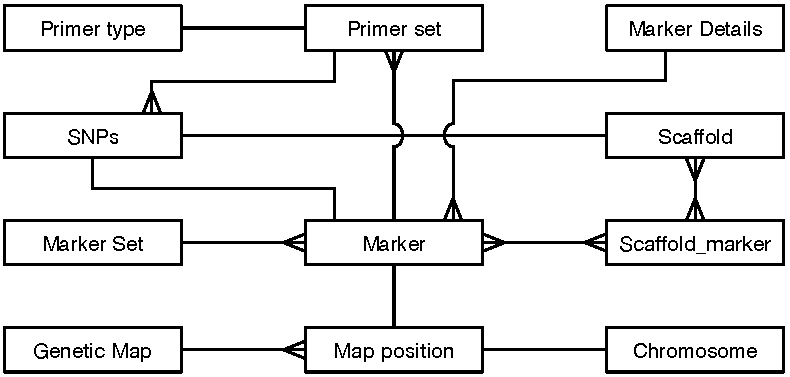
\includegraphics[width=1\textwidth]{Conclusions/Figures/GenetiMapTables.pdf}
\caption{Tables to store information about genetic maps.}
\label{fig:discussion:geneticMapsTables}
\end{figure}

Genetic maps are produced from the genotype of several markers (marker sets). 
Those markers can be developed explicitly for the genetic map or from an already published marker set, usually in the form of an SNP array. 
A database containing several genetic maps should be able to distinguish the origin of the used markers.
However, a genetic map may contain markers from several marker sets.
For those reasons, a genetic map is not connected directly to a marker set, but the relationship is maintained trough the markers and their position in the genetic map.

To be able to use the genetic marker in a genomic context, the sequence of the markers must be mapped to a reference. 
The assembly may be in a single pseudomolecule or in separated scaffolds. 
If the assembly is fragmented, the  map can be used to anchor the scaffolds to a genetic position. 
If the assembly consist on long scaffolds the genetic map and the positions can be used to find if a rearrangement event has occurred in the lines used for the map. 
If a rearrangement is present, the collinearity between the genomic and genetic reference is not conserved. 
Having the markers and scaffolds in the database simplifies this kind of analysis, as all the needed data is readily available. 

Furthermore, PolyMarker (Chapter \ref{cha:polymarker}) has been used to design KASP assays for most of the primers in the 90k \citep{Wang2014} and 820k \citet{Winfield2016} SNP arrays. 
The primers for the assays can be integrated in the database. 
\unsure{Do we have any paper on the lab where this approach is used?}
This allows to envision a use case where known flanking markers are queried and the database can return a list of possible markers with the primers already designed to be validated on a mapping population. 

\section{Integration of different genome references. }

The efforts to produce a wheat reference genome had been focused on the \gls{cs} variety. 
\acrshort{cs} is only cultivated as a research line, as it is susceptible to several pathogens and its yield is inferior to modern varieties.  
The reason for \acrshort{cs} to be the selected cultivar to be sequenced as reference is historic: it has long been a variety  for research.
\acrshort{cs} was originally chosen because it was able to cross with rye. 
It has also been used to produce lines with chromosomic aberrations, useful to find if any particular chromosome is responsible for certain traits \citep{Sears1985}. 

New assemblies are required to address the shortcomings of the use of \acrshort{cs} as a genome reference and to include the diversity from other lines \citep{Allen2016,Winfield2016}. 
The assemblies may include their own annotation, and that should be reflected in the database too. 

As of September 2016 there are four sets of genomic sequence used by the wheat community:
\begin{enumerate}
	\item  A 454 whole genome shotgun sequence that is unassembled, and each read is treated as a scaffold \citep{Brenchley2012}.
	\item The genome assembly and annotation from the \gls{css} done by the \acrshort{iwgsc} \citep{Mayer2014}.
	\item A whole genome shotgun sequence from a syntetic wheat, without a corresponding annotation \citep{Chapman2015}.
	\item The whole genome shotgun sequencing and annotation from \acrshort{cs} (TGACv1; \citealt{Clark2016}).
\end{enumerate}

All those references can be aligned to each other to find corresponding region. 
The corresponding regions can be stored in the scaffold mapping table. 
Furthermore, the scaffolds can be mapped to relative species, such as \textit{Brachypodium distachyon}, \textit{Oryza sativa}, \textit{Sorghum bicolor}, and \textit{Hordeum vulgare} to find synthenic blocks. 

As each genome assemblies are usually annotated with their genes and other features. 
To include the annotation, each scaffold can contain several features. 
As some features consist on sub-features, like genes conformed by several exons, a recursive relationship is included in the features tables. 
With the support of scaffold mapping, the different annotations can be projected on different references. 
Gene models, like the ones described in \citep{Krasileva2013}, and  genetic markers can be aligned to any of the reference genomes.

With all those relationships available, the \textit{in silico} mapping in Chapter \ref{yr15} could be produced on several references at once. 
Also, the relationship between different gene models could be simplified, as the corresponding features will share coordinates.
Likewise, the co-expression of genes located in the same region could be an useful feature for expVIP (Chapter \ref{cha:exp}). 

Figure \ref{fig:discussion:assemblyTables} include the tables used to store assemblies, the relationships between them and their annotation. 

\begin{figure}
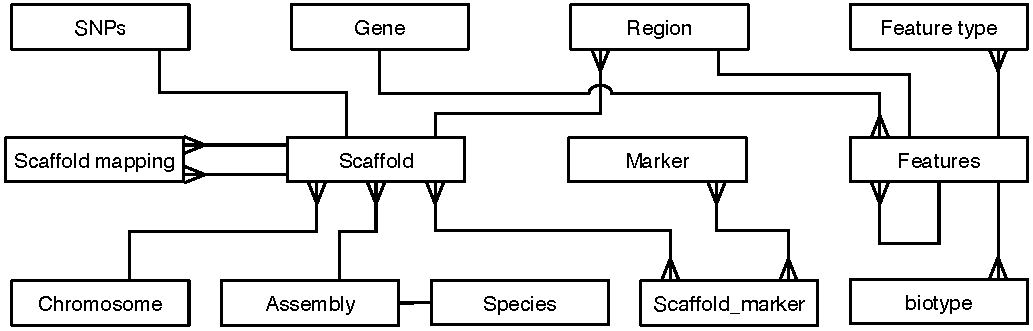
\includegraphics[width=1\textwidth]{Conclusions/Figures/assemblyTables.pdf}
\caption{Tables to store information about genome assemblies and their annotation.}
\label{fig:discussion:assemblyTables}
\end{figure}

\section{Integration with other services}
Currently, the publicly available wheat resources are scattered as supplemental materials on their corresponding publication or available as ad hoc systems focused on a particular field.
For example ensembl has two different views for every organism: from the genomic point of view and from the expression data. 
The Collaborative Open Plant Omics (COPO; \citealt{Davey2015}) is trying to integrate different sources and types of data by connecting the data providers. 
This approach requires the cooperation of the service providers, which have their own view of what is important. 
I believe that in order to effectively integrate the resources it is necessary to understand how the users are likely to interact with the data.


\section{Side projects}

PolyInDel / . 

\section{Final remarks}

In order to produce bioinformatics software that is powerful and usable it is required an understanding of both: the biological processes to solve on one hand, and the computational methods and software best development practices on the other.
